\chapter{Skup podataka}
\label{chp:dataset}

Za analizu podataka i razvoj modela proučavani su samo trokuti. Naime, ako neke pravilnosti nisu uočene na trokutima ili ako neki model ciljnu varijablu ne predviđa dobro na trokutima, onda se ta pravilnost i taj model ne mogu generalizirati jer specijalno ne vrijede na trokutima. Također, zbog korolara~\ref{cor:spectrum_similar_domains} i propozicije~\ref{prop:diameter_polygon} svi su trokuti dijametra $ \numprint{1} $.

\par

\section{Izrada skupa podataka}
\label{sec:generate_dataset}

Izlaz svakog generatora trokuta matrica je oblika
\begin{equation*}
    \begin{pmatrix}
        x_{\numprint{1} , \numprint{1}} & y_{\numprint{1} , \numprint{1}} & x_{\numprint{1} , \numprint{2}} & y_{\numprint{1} , \numprint{2}} & x_{\numprint{1} , \numprint{3}} & y_{\numprint{1} , \numprint{3}} \\
        x_{\numprint{2} , \numprint{1}} & y_{\numprint{2} , \numprint{1}} & x_{\numprint{2} , \numprint{2}} & y_{\numprint{2} , \numprint{2}} & x_{\numprint{2} , \numprint{3}} & y_{\numprint{2} , \numprint{3}} \\
        \vdots & \vdots & \vdots & \vdots & \vdots & \vdots \\
        x_{N , \numprint{1}} & y_{N , \numprint{1}} & x_{N , \numprint{2}} & y_{N , \numprint{2}} & x_{N , \numprint{3}} & y_{N , \numprint{3}}
    \end{pmatrix}
    \in \MatrixAlgebramn{\reals}{N}{\numprint{6}} \text{,}
\end{equation*}
gdje je $ N \in \positives{\naturals} $ broj generiranih trokuta, a $ \left( x_{i j} , y_{i j} \right) \in \reals^{\numprint{2}} $ koordinate $ j $-tog vrha $ i $-tog trokuta, za svake $ \left( i , j \right) \in \left\{ \numprint{1} , \numprint{2} , \dotsc , N \right\} \times \left\{ \numprint{1} , \numprint{2} , \numprint{3} \right\} $. Zajamčeno je da je svaki generirani trokut dijametra $ \numprint{1} $ (do na numeričku točnost prikaza i računa realnih brojeva na računalu), da su vrhovi enumerirani u pozitivnom smjeru i da je prvi vrh trokuta onaj s najmanjom vrijednosti ordinate (i najvećom vrijednosti apscise ako više vrhova ima istu i najmanju vrijednost ordinate). Za programe i modele koji zahtijevaju/pretpostavljaju dodatno određeni položaj trokuta u odnosu na ishodište koordinatnog sustava, i taj se zahtjev zadovoljava već kod generatora (i ne pripada pretprocesiranju podataka; dakle, vrijeme potrebno za takvu standardizaciju ne ulazi u mjereno vrijeme).

\par

Trokuti su generirani ekvidistantnom diskretizacijom pravokutnika $ \intervalcc{\numprint{0}}{\frac{\numprint{1}}{\numprint{2}}} \times \intervalcc{\numprint{0}}{\frac{\sqrt{\numprint{3}}}{\numprint{2}}} \subseteq \reals^{\numprint{2}} $ i zatim biranjem onih točaka u toj mreži koje pripadaju skupu $ D_{{\bigtriangleup}} $ iz propozicije~\ref{prop:triangle_characteristic_bijective}. Ipak, zbog ograničenja programa za numerički račun \emph{odbačene} su one točke čija vrijednost ordinate ne iznosi barem $ \numprint{0.05} $. Inicijalna diskretizacija interval $ \intervalcc{\numprint{0}}{\frac{\numprint{1}}{\numprint{2}}} $ podijelila je na $ \numprint{1001} $ točku ($ \numprint{1000} $ podintervala), a interval $ \intervalcc{\numprint{0}}{\frac{\sqrt{\numprint{3}}}{\numprint{2}}} $ na $ \numprint{1733} $ točke ($ \numprint{1732} $ podintervala). Time je (nakon \emph{odbacivanja} točaka) dobiven $ \numprint{1129741} $ trokut (za svaki trokut uzeti su vrhovi $ \left( \frac{\numprint{1}}{\numprint{2}} , \numprint{0} \right) , V , \left( {- \frac{\numprint{1}}{\numprint{2}}} , \numprint{0} \right) $, gdje je $ V \in \reals^{\numprint{2}} $ odgovarajuća generirana točka).

\par

\begin{figure}[htb!]
    \centering
    \begin{subfigure}{69.5mm}
        \centering
        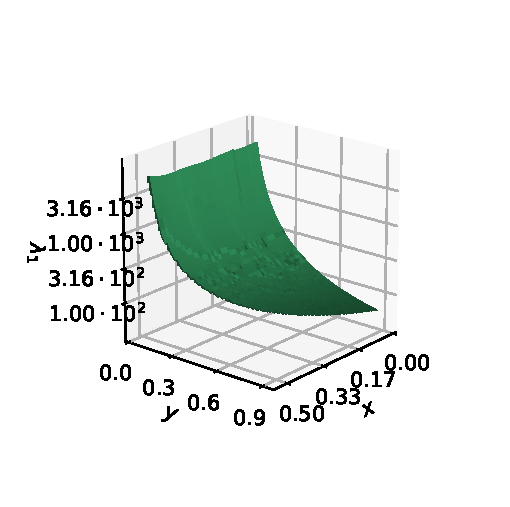
\includegraphics[width = 64.5mm]{figures/eigenvalues_3D.pdf}
        \caption{Prostorni pogled}
        \label{fig:triangles_eigenvalues_spatial}
    \end{subfigure}
    \begin{subfigure}{74mm}
        \centering
        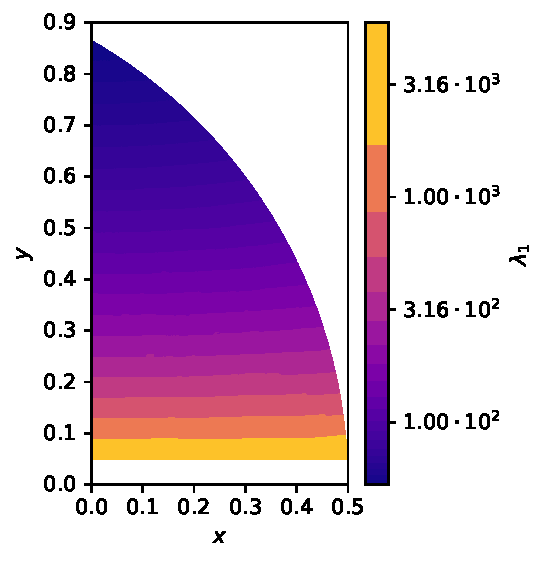
\includegraphics[width = 69mm]{figures/eigenvalues.pdf}
        \caption{Tlocrtni pogled}
        \label{fig:triangles_eigenvalues_contour}
    \end{subfigure}
    \caption[Najmanje svojstvene vrijednosti Laplaceovog operatora na trokutima]{Najmanje svojstvene vrijednosti Laplaceovog operatora na trokutima. Slike prikazuju funkciju koja točki \ensuremath{V \in D_{{\bigtriangleup}}}, gdje je \ensuremath{D_{{\bigtriangleup}}} skup iz propozicije~\ref{prop:triangle_characteristic_bijective}, pridružuje najmanju svojstvenu vrijednost Laplaceovog operatora na otvorenom trokutu čiji su vrhovi \ensuremath{\left( \frac{\numprint{1}}{\numprint{2}} , \numprint{0} \right) , V , \left( {- \frac{\numprint{1}}{\numprint{2}}} , \numprint{0} \right)}. Iz tehničkih razloga svojstvene vrijednosti na točkama \emph{ispod} pravca \ensuremath{y = \numprint{0.05}} nije bilo moguće izračunati, ali vrijednosti neograničeno rastu kada vrijednost ordinate teži u \ensuremath{\numprint{0}}. Najmanja prikazana vrijednost iznosi \ensuremath{\numprint{52.7248}}, a najveća \ensuremath{\numprint{5938.1931}} (vrijednosti su na dijagramima prikazane u logaritamskoj skali).}
    \label{fig:triangles_eigenvalues}
\end{figure}

\par%
\clearpage%
\newpage

Originalni skup trokuta nije pogodan za konstrukciju modela. Naime, kao što je vidljivo iz slike~\ref{fig:triangles_eigenvalues}, rast najmanje svojstvene vrijednosti vrlo je brz s obzirom na pad vrijednosti ordinate trećeg vrha trokuta pa je zbog ekvidistantnosti mreže neproporcionalno više točaka u skupu $ D_{{\bigtriangleup}} $ generirano s \emph{većom} najmanjom svojstvenom vrijednosti. Skup podataka stoga je potrebno prvo \emph{uravnotežiti}\footnote{Zapravo, legitimno je tvrditi da je realna situacija da su \emph{ekstremno velike} najmanje svojstvene vrijednosti puno zastupljenije nego \emph{manje} jer, kada bi se uniformno slučajno birala točka u skupu $ D_{{\bigtriangleup}} $ iz propozicije~\ref{prop:triangle_characteristic_bijective}, veća je vjerojatnost da će najmanja svojstvena vrijednost Laplaceovog operatora na dobivenom trokutu biti \emph{velika} nego da će biti \emph{mala}. Međutim, za konstrukciju modela strojnog učenja poželjno je da se on ne \emph{pretrenira} na velikim vrijednostima, nego da dobro predviđa i manje vrijednosti. Relativno mala greška na \emph{ekstremno velikim} vrijednostima velika je greška na \emph{malim} vrijednostima, stoga bi neuravnotežena zastupljenost \emph{ekstremno velikih} vrijednosti mogla katastrofalno utjecati na uspješnost modela na \emph{malim} vrijednostima.}.

\par

\begin{remark} \label{rem:point_Laplacian_eigenvalue}
    U daljnjem tekstu, kada će se spominjati najmanja svojstvena vrijednost Laplaceovog operatora u kontekstu s jedinstvenom točkom odnosno njezinom vrijednosti apscise i/ili ordinate (na primjer, ovisnost najmanje svojstvene vrijednosti Laplaceovog operatora o vrijednosti ordinate), tada će se, zapravo, govoriti o preslikavanju sa slike~\ref{fig:triangles_eigenvalues}.
\end{remark}

\par

\subsection{Uravnoteženje podataka}

\par

Na slici~\ref{fig:triangles_eigenvalues} vidljivo je da je najmanja svojstvena vrijednost relativno konstantna za konstantnu vrijednost ordinate (za razliku od varijabilnosti s obzirom na fiksiranu vrijednost apscise). Stoga je generiran pomoćni skup trokuta, takav da je interval $ \intervalcc{\numprint{0}}{\frac{\sqrt{\numprint{3}}}{\numprint{2}}} $ diskretiziran opet istim točkama kao u prvom slučaju, a za svaku vrijednost $ y_{j} $ te diskretizacije dužina dobivena presjekom skupa $ D_{{\bigtriangleup}} $ i pravca $ y = y_{j} $ ekvidistantno je podijeljena na $ \numprint{5} $ točaka. Točnije, generirane su vrijednosti na krivuljama
\begin{equation*}
    x = p \left( {- \frac{\numprint{1}}{\numprint{2}}} + \sqrt{\numprint{1} - y^{\numprint{2}}} \right) , \quad p \in \left\{ \numprint{0} , \frac{\numprint{1}}{\numprint{4}} , \frac{\numprint{1}}{\numprint{2}} , \frac{\numprint{3}}{\numprint{4}} , \numprint{1} \right\}
\end{equation*}
(tako da je $ \left( p^{{- \numprint{1}}} x + \frac{\numprint{1}}{\numprint{2}} \right)^{\numprint{2}} + y^{\numprint{2}} = \numprint{1} $ ako je $ p \neq \numprint{0} $; inače je, očito, $ x = \numprint{0} $) u skupu $ D_{{\bigtriangleup}} $, u onim vrijednostima $ y \in \intervaloc{\numprint{0}}{\frac{\sqrt{\numprint{3}}}{\numprint{2}}} $ iz originalne ekvidistantne mreže. U tim su točkama (trokutima) ponovo izračunate najmanje svojstvene vrijednosti.

\par

Za svaki generirani trokut (u originalnom skupu podataka i u pomoćnom) izračunate su duljine stranica, veličine vanjskih kutova, singularne vrijednosti duljina stranica, singularne vrijednosti vanjskih kutova i, naravno, najmanja svojstvena vrijednost Laplaceovog operatora. \emph{Spojimo} te vrijednosti u vektor (redak tablice) i označimo skup takvih zapisa o trokutima (tablicu) na prvotnom skupu s $ A $, a na pomoćnom skupu s $ B $. Elemente skupova $ A $ i $ B $ označavat ćemo s $ \asvector{t} $---svaki takav element vektor je informacija o trokutu---a \emph{zapis} o najmanjoj svojstvenoj vrijednosti u vektoru $ \asvector{t} $ označavat ćemo s $ \asvector{t}{\text{\texttt{[}} \lambda \text{\texttt{]}}} $. Označimo i multiskupove
\begin{align*}
    A{\text{\texttt{[}} \lambda \text{\texttt{]}}} & \coloneqq \left\{ \asvector{t}{\text{\texttt{[}} \lambda \text{\texttt{]}}} : \asvector{t} \in A \right\} \text{,} \\
    B{\text{\texttt{[}} \lambda \text{\texttt{]}}} & \coloneqq \left\{ \asvector{t}{\text{\texttt{[}} \lambda \text{\texttt{]}}} : \asvector{t} \in B \right\} \text{.}
\end{align*}

\par

Tada su izračunate vrijednosti kvantila dvadesetina $ \lambda_{\numprint{0.00}} \leq \lambda_{\numprint{0.05}} \leq \lambda_{\numprint{0.10}} \leq \dotsb \leq \lambda_{\numprint{1.00}} $ skupa $ B{\text{\texttt{[}} \lambda \text{\texttt{]}}} $ (zapravo je, dodatno, uzeto $ \lambda_{\numprint{0.00}} = \min \left( A{\text{\texttt{[}} \lambda \text{\texttt{]}}} \cup B{\text{\texttt{[}} \lambda \text{\texttt{]}}} \right) - \varepsilon $ i $ \lambda_{\numprint{1.00}} = \max \left( A{\text{\texttt{[}} \lambda \text{\texttt{]}}} \cup B{\text{\texttt{[}} \lambda \text{\texttt{]}}} \right) + \varepsilon $ za neki $ \varepsilon > \numprint{0} $). S ovim vrijednostima skup $ A $ je particioniran na skupove $ A_{\numprint{0.05}} , A_{\numprint{0.10}} , \dotsc , A_{\numprint{1.00}} \subseteq A $ definirane s
\begin{equation*}
    A_{p} \coloneqq \left\{ \asvector{t} \in A : \lambda_{p - \numprint{0.05}} \leq \asvector{t}{\text{\texttt{[}} \lambda \text{\texttt{]}}} < \lambda \right\} \subseteq A , \quad \forall p \in \left\{ \numprint{0.05} , \numprint{0.10} , \dotsc , \numprint{1.00} \right\} \text{,}
\end{equation*}
Dobiveni skup $ A_{\numprint{0.95}} $ bio je najveći, i to više od $ \numprint{15} $ puta veći nego $ A_{\numprint{0.05}} $, koji je bio najmanji. S druge strane, kako su granice definiranih skupova zapravo granice jednako velikih kvantila multiskupa $ B{\text{\texttt{[}} \lambda \text{\texttt{]}}} $, tako definirani dijelovi skupa $ B $ bili bi podjednako veliki. Dijelovi skupa $ D_{{\bigtriangleup}} $ na slici~\ref{fig:triangles_eigenvalues_contour} zapravo su obojani s obzirom na najmanju svojstvenu vrijednost Laplaceovog operatora u $ \numprint{20} $ nijansi od kojih svaka pripada jednom od kvantilnih intervala $ \intervalco{\lambda_{p - \numprint{0.05}}}{\lambda_{p}} $.

\par

Konačno je, za zadani $ n \in \positives{\naturals} $, iz svakog od skupova $ A_{\numprint{0.05}} , A_{\numprint{0.10}} , \dotsc , A_{\numprint{1.00}} $ slučajnim odabirom uzeto po $ n $ različitih zapisa, čime je konstruiran treći, novi skup $ A ' \subseteq A $. Pritom se zahtijevalo da varijanca svake kategorije podataka u izabranom podskupu $ A_{p} ' $ skupa $ A_{p} \in \left\{ A_{\numprint{0.05}} , A_{\numprint{0.10}} , \dotsc , A_{\numprint{1.00}} \right\} $ ostane što sličnija varijanci te kategorije podataka u skupu $ A_{p} $.

\par

Na slici~\ref{fig:dataset_balanced_discretisation} prikazan je rezultat opisanog postupka za $ n = \numprint{50} $ (ukupno $ \numprint{1000} $ točaka, u odnosu na originalnih $ \numprint{1129741} $).

\par

\begin{figure}[htb!]
    \centering
    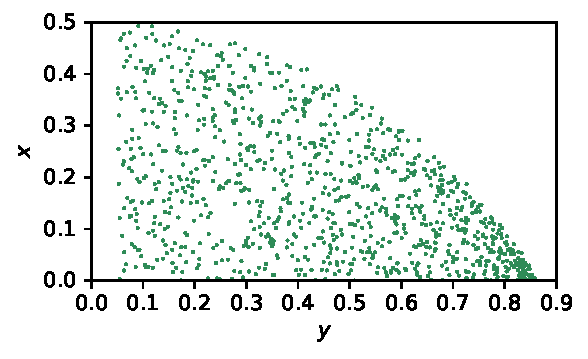
\includegraphics[width = 80mm]{figures/sample.pdf}
    \caption{\emph{Uravnotežena} diskretizacija skupa \ensuremath{D_{{\bigtriangleup}}} iz propozicije~\ref{prop:triangle_characteristic_bijective}}
    \label{fig:dataset_balanced_discretisation}
\end{figure}

\par

\section{Izrada skupa podataka za treniranje, validaciju i testiranje}
\label{sec:dataset_split}

Osnovna ideja bila je predodrediti $ {{\sim} \unit[\numprint{70}]{\%}} $ podataka za treniranje, $ {{\sim} \unit[\numprint{15}]{\%}} $ podataka za validaciju i $ {{\sim} \unit[\numprint{15}]{\%}} $ podataka za testiranje. Kod modela kod kojih validacija nije potrebna---zapravo, samo kod linearne regresije---podatci za validaciju spojeni su s podatcima za testiranje u veći skup podataka za testiranje, koji čini $ {{\sim} \unit[\numprint{30}]{\%}} $ svih podataka.

\par

\subsection{Izrada skupa podataka za treniranje, validaciju i testiranje za modele s isključivo numeričkim ulaznim podatcima}

\par

Kako sva korištena numerička obilježja trokuta (poligona) ne ovise o položaju, orijentaciji i rotaciji trokuta u ravnini, kod izrade skupova podataka za modele koji primaju isključivo numeričke podatke nije bilo potrebno generirati više reprezentanata sličnih trokuta (zapravo, sukladnih jer su svi trokuti istog dijametra). Stoga je za takve modele bilo moguće s istim brojem podataka obuhvatiti veći broj slučajeva.

\par

Opisanom metodom za uravnoteženje podataka ukupni skup podataka za ove modele dobiven je tako da se iz skupa $ A_{p} $ biralo $ \min \left( \left\{ \card \left( A_{\numprint{0.00}} \right) , \card \left( A_{\numprint{0.05}} \right) , \dotsc , \card \left( A_{\numprint{1.00}} \right) \right\} \right) $ podataka, za svaki $ p \in \left\{ \numprint{0.00} , \numprint{0.05} , \dotsc , \numprint{1.00} \right\} $. Tada je na dobivenom skupu $ A ' $ ponovljen postupak tako da se dobije skup $ A '' $ čiji je kardinalitet otprilike $ \unit[\numprint{30}]{\%} $ kardinaliteta skupa $ A ' $, ali ovdje se što vjernija varijanca (što sličnija varijanci na $ A_{p} ' $, a ne prvotnoj na $ A_{p} $) pokušala zadržati ne samo na $ A_{p} '' $, nego i na $ A_{p} ' \setminus A_{p} '' $. Na kraju se na skupu $ A '' $ isti postupak ponovio generirajući skup $ A ''' $ kardinaliteta upola manjeg nego $ A '' $, pri čemu se i ovdje originalna varijanca (varijanca iz skupa $ A_{p} '' $, a ne iz $ A_{p} ' $ ili $ A_{p} $) zadržavala na biranim dijelovima i na njihovim komplementima. Tako dobiveni skupovi su
\begin{enumerate}
    \item skup podataka za treniranje: $ A ' \setminus A '' $---ukupno $ \numprint{76280} $ trokuta,
    \item skup podataka za validaciju: $ A '' \setminus A ''' $---ukupno $ \numprint{16340} $ trokuta,
    \item skup podataka za testiranje: $ A ''' $---ukupno $ \numprint{16340} $ trokuta.
\end{enumerate}

\par

\subsection{Izrada skupa podataka za treniranje, validaciju i testiranje za modele s vizualnim ulaznim podatcima}

Budući da vizualna karakterizacija poligona ovisi o njegovu položaju, rotaciji i orijentaciji, za generiranje reprezentativnog skupa podataka s vizualnim karakterizacijama bilo je potrebno uključiti pojedine perturbacije trokuta. Tako je originalni skup podataka prvo povećan dodavanjem refleksija oko ordinate svih trokuta (uključujući i jednakokračnih i jednakostraničnog, iako su oni simetrični), a zatim rotiranjem svakog trokuta $ \numprint{10} $ puta za pseudoslučajno izabrani kut. Trokuti su bili rotirani neovisno jedan o drugme, štoviše, svaka od $ \numprint{10} $ rotacija svakog trokuta bila je neovisna o drugim rotacijama. Kut rotacije birao se uniformno pseudoslučajno iz skupa $ \intervalco{\numprint{0}}{\numprint{2} \pi} $. Konačno je opisanim postupkom dobiveno $ \numprint{22594820} $ trokuta. Ovi su trokuti zatim translatirani tako da im središte upisane kružnice bude u ishodištu (u točki $ \left( 0 , 0 \right) $).

\par

Dobiveni je skup tada bio reduciran do uravnoteženog skupa $ A ' $ od \emph{svega} $ \numprint{100000} $ trokuta (zbog ograničenih resursa varijanca se računala samo na singularnim vrijednostima duljina stranica i vanjskih kutova i na najmanjim svojstvenim vrijednostima Laplaceovog operatora). Zatim su, analognim postupkom kao kod generiranja skupa podataka za modele s isključivo numeričkim ulaznim podatcima, ekstrahirani skupovi za validaciju $ A '' \setminus A ''' $ i testiranje $ A ''' $ (ovdje su se uzimale u obzir varijance svih obilježja i ciljne varijable). Konačni kardinaliteti skupova iznosili su
\begin{enumerate}
    \item skup podataka za treniranje: $ A ' \setminus A '' $---ukupno $ \numprint{70000} $ trokuta,
    \item skup podataka za validaciju: $ A '' \setminus A ''' $---ukupno $ \numprint{15000} $ trokuta,
    \item skup podataka za testiranje: $ A ''' $---ukupno $ \numprint{15000} $ trokuta.
\end{enumerate}

\par

\section{Eksploratorna analiza numeričkih podataka}
\label{sec:dataset_exploratory_analysis}

U eksploratornoj analizi podataka postupkom uravnotežavanja podataka iz numeričkog skupa podataka za treniranje ekstrahirano je $ \numprint{1000} $ točaka (po $ \numprint{50} $ iz svakog dijela) za vizualizaciju komentiranih zavisnosti radi bolje preglednosti. Kako su dijagrami bili gotovo isti pri svakom novom generiranju takvog podskupa, rezultati koji su predstavljeni vizualno su reprezentativni. Ipak, osim vizualizacije predstavljene su i numeričke vrijednosti koje su izračunate na cijelom skupu podataka za treniranje.

\par

Iako stvarna najmanja svojstvena vrijednost ima \emph{jako} konveksan oblik i brz rast s obzirom na pad ordinate (\seetxt~sliku~\ref{fig:triangles_eigenvalues}), njezin multiplikativni inverz gotovo pa je linearan s obzirom na vrijednost ordinate---Pearsonov koeficijent korelacije iznosi čak $ \unit[\numprint{99.8239}]{\%} $, što je najveći opaženi koeficijent korelacije (po apsolutnoj vrijednosti). S druge strane, za \emph{relativno fiksnu} vrijednost ordinate (zadanu da bude u nekom \emph{užem} intervalu), multiplikativni inverz najmanje svojstvene vrijednosti opada u blagom luku s porastom vrijednosti apscise. Ove su ovisnosti prikazane na slici~\ref{fig:x_y_eigenvalue}.

\par%
\clearpage%
\newpage

\begin{figure}[htb!]
    \centering
    \begin{subfigure}{51.4mm}
        \centering
        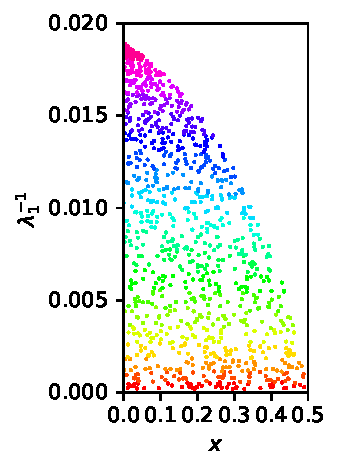
\includegraphics[width = 46.4mm]{figures/x-lambda.pdf}
        \caption{Apscisa}
        \label{fig:x_y_eigenvalues_abscissa}
    \end{subfigure}
    \begin{subfigure}{76.2mm}
        \centering
        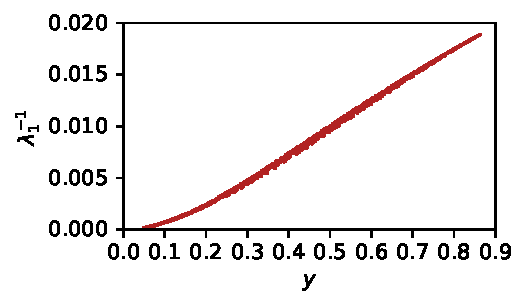
\includegraphics[width = 71.2mm]{figures/y-lambda.pdf}
        \caption{Ordinata}
        \label{fig:x_y_eigenvalues_ordinate}
    \end{subfigure}
    \caption[Ovisnosti multiplikativnog inverza najmanje svojstvene vrijednosti Laplaceovog operatora na trokutima dijametra \ensuremath{\numprint{1}} u odnosu na koordinate karakterističnih točaka iz propozicije~\ref{prop:triangle_characteristic_bijective}]{Ovisnosti multiplikativnog inverza najmanje svojstvene vrijednosti Laplaceovog operatora na trokutima dijametra \ensuremath{\numprint{1}} u odnosu na koordinate karakterističnih točaka iz propozicije~\ref{prop:triangle_characteristic_bijective}. Na slici~\ref{fig:x_y_eigenvalues_abscissa} točke su obojane s obzirom na vrijednosti ordinate po kvantilima zastupljenosti u skupu podataka za treniranje.}
    \label{fig:x_y_eigenvalue}
\end{figure}

\par

Kao što je vidljivo na slici~\ref{fig:triangles_eigenvalues}, na bilo kojoj kružnici sa središtem u točki $ \left( {- \frac{\numprint{1}}{\numprint{2}} } , \numprint{0} \right) $, koja sa skupom $ D_{{\bigtriangleup}} $ ima zajedničkih točaka, svojstvene vrijednosti pojavljuju se u nekom samo slijeva ograničenom intervalu. Radijus takvih kružnica zapravo je duljina druge najdulje stranice trokuta koje te točke u skupu $ D_{{\bigtriangleup}} $ predstavljaju, stoga je jasno da najmanja svojstvena vrijednost Laplaceovog operatora nema izraženu korelaciju s drugom najduljom stranicom trokuta. Isto tako, svim trokutima najdulja je stranica duljine $ \numprint{1} $ pa korelacija najmanje svojstvene vrijednosti i duljine najdulje stranice (za trokute fisknog dijametra) uopće ne postoji. Tek je postojeća korelacija s duljinom najkraće stranice, kao što je vidljivo na slici~\ref{fig:edge_angle_eigenvalue}, a čiji Pearsonov koeficijent korelacije iznosi $ \unit[\numprint{94.8912}]{\%} $. Na toj su slici prikazane i ovisnosti o vanjskim kutovima, od čijih korelacija valja spomenuti korelaciju s najvećim vanjskim kutom (suplementom najmanjeg unutarnjeg kuta), čiji Pearsonov koeficijent korelacije iznosi $ {- \unit[\numprint{97.8601}]{\%}} $.

\par%
\clearpage%
\newpage

\begin{figure}[htb!]
    \centering
    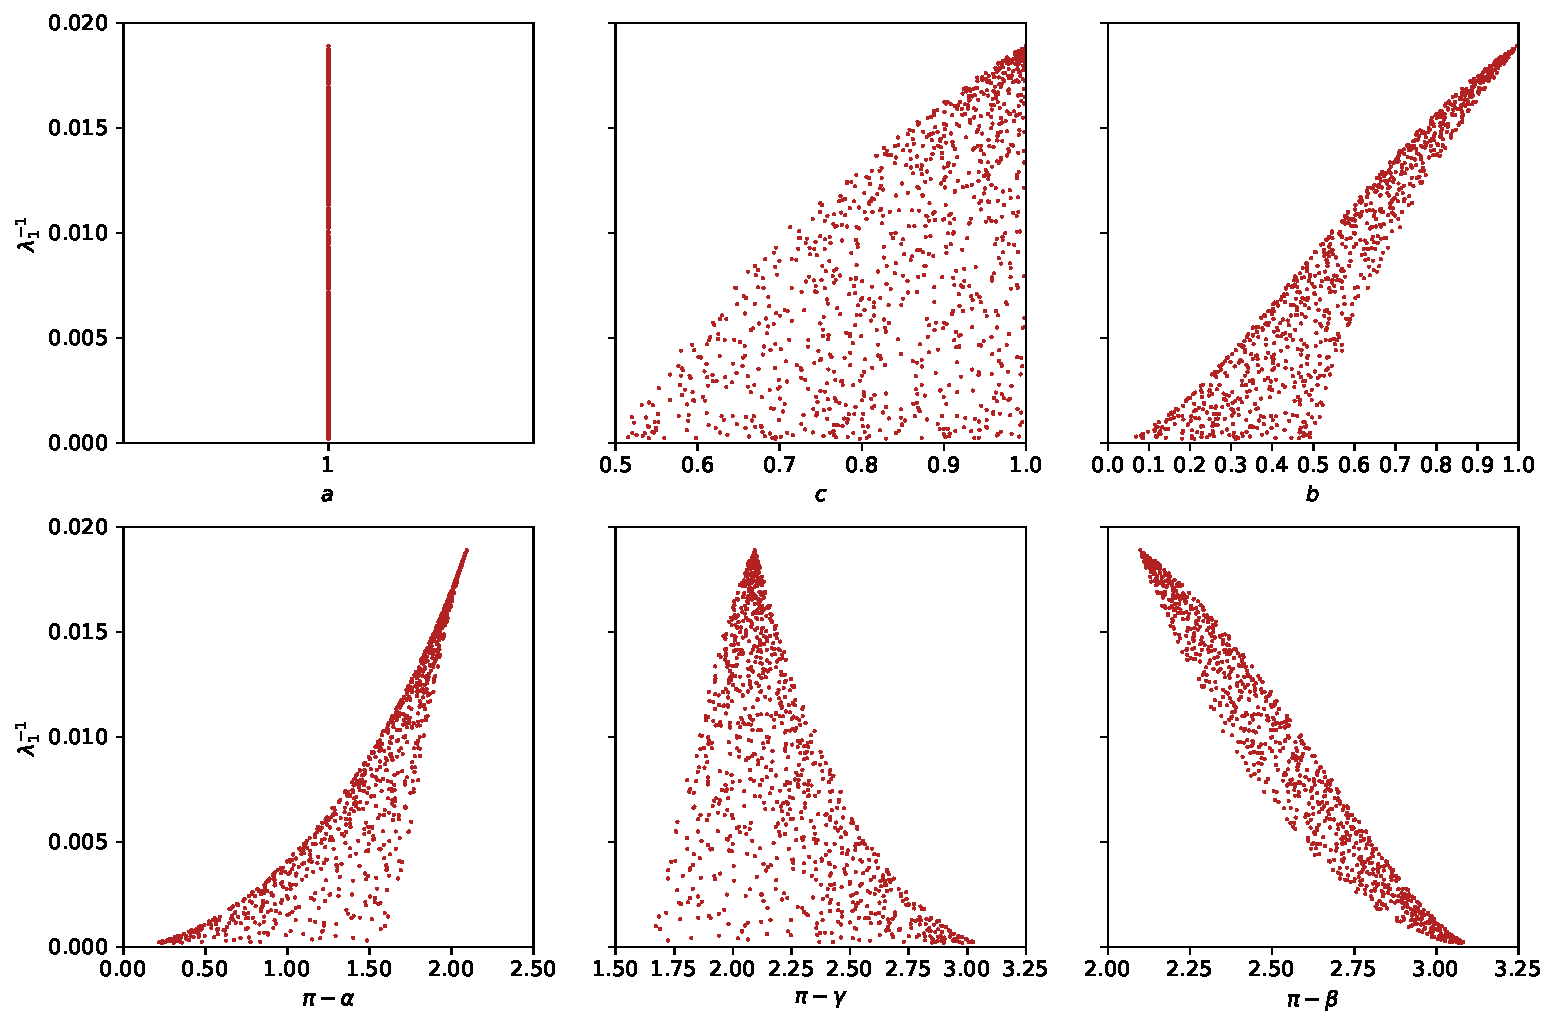
\includegraphics[width = 132mm]{figures/edge_angle-lambda.pdf}
    \caption[Ovisnosti multiplikativnog inverza najmanje svojstvene vrijednosti Laplaceovog operatora na trokutima dijametra \ensuremath{\numprint{1}} u odnosu na duljine stranica i veličine vanjskih kutova]{Ovisnosti multiplikativnog inverza najmanje svojstvene vrijednosti Laplaceovog operatora na trokutima dijametra \ensuremath{\numprint{1}} u odnosu na duljine stranica i veličine vanjskih kutova. Duljine stranica trokuta označene su tako da je \ensuremath{a \geq c \geq b}, a unutarnji kutovi tako da je \ensuremath{\alpha \geq \gamma \geq \beta} (vanjski kutovi su tada \ensuremath{\pi - \alpha \leq \pi - \gamma \leq \pi - \beta}).}
    \label{fig:edge_angle_eigenvalue}
\end{figure}

\par

Slično kao što je korelacija najmanje svojstvene vrijednosti s duljinom najdulje stranice nepostojeća zbog fiksne duljine najdulje stranice, uzimajući u obzir slutnju~\ref{conj:polygon_characteristic_angle_fixed} za očekivati je i da je nepostojeća korelacija s najvećom singularnom vrijednosti vanjskih kutova. Međutim, ovdje je ta korelacija nepostojeća čak i ako dijametar trokuta nije fiksan jer vanjski kutovi ne ovise o dijametru poligona. Također, zbog slutnje~\ref{conj:polygon_characteristic_number_of_values} za očekivati je da je dovoljno proučavati samo dvije najveće singularne vrijednosti duljina stranica i vanjskih kutova, a ne sve tri (ako uopće ima smisla proučavati najveću singularnu vrijednosti vanjskih kutova). Ovisnosti najmanje svojstvene vrijednosti o ovim singularnim vrijednostima prikazane su na slici~\ref{fig:singular_value_eigenvalue}.

\par

Osim najveće singularne vrijednosti vanjskih kutova, sve ostale singularne vrijednosti s multiplikativnim inverzom najmanje svojstvene vrijednosti Laplaceovog operatora imaju Pearsonov koeficijent korelacije po apsolutnoj vrijednosti veći od $ \unit[\numprint{90}]{\%} $. Koeficijenti iznose: $ \unit[\numprint{99.1195}]{\%} $ za najveću singularnu vrijednost duljina stranica---što je najveća korelacija (po apsolutnoj vrijednosti) izuzev korelacije vrijednosti ordinate i korelacija kasnije spomenutih složenih značajki---$ {- \unit[\numprint{93.3544}]{\%}} $ za drugu i treću najveću singularnu vrijednost duljina stranica i $ {- \unit[\numprint{94.6484}]{\%}} $ za drugu i treću najveću singularnu vrijednost vanjskih kutova.

\par

\begin{figure}[htb!]
    \centering
    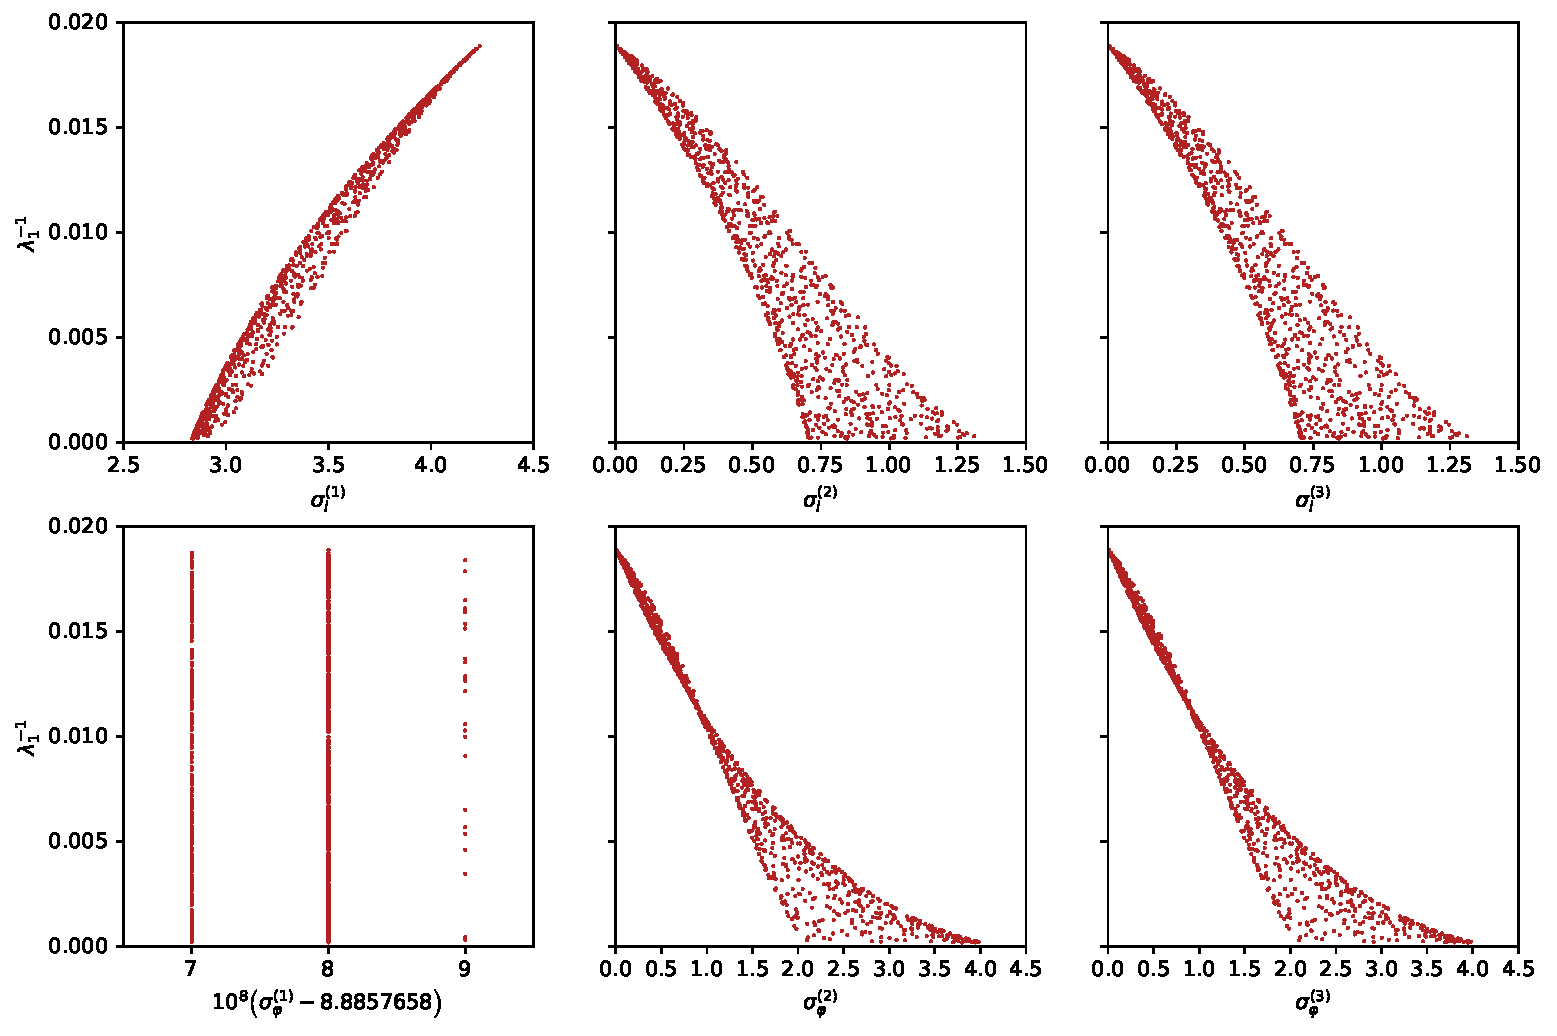
\includegraphics[width = 132mm]{figures/sv-lambda.pdf}
    \caption[Ovisnosti multiplikativnog inverza najmanje svojstvene vrijednosti Laplaceovog operatora na trokutima dijametra \ensuremath{\numprint{1}} u odnosu na singularne vrijednosti duljina stranica i vanjskih kutova]{Ovisnosti multiplikativnog inverza najmanje svojstvene vrijednosti Laplaceovog operatora na trokutima dijametra \ensuremath{\numprint{1}} u odnosu na singularne vrijednosti duljina stranica i vanjskih kutova. Vektor \ensuremath{\sigma_{l} = \left( \sigma_{l}^{\left( \numprint{1} \right)} , \sigma_{l}^{\left( \numprint{2} \right)} , \sigma_{l}^{\left( \numprint{3} \right)} \right) \in \intervalco{\numprint{0}}{{+ \infty}}^{\numprint{3}}} vektor je singularnih vrijednosti duljina stranica, a vektor \ensuremath{\sigma_{\varphi} = \left( \sigma_{\varphi}^{\left( \numprint{1} \right)} , \sigma_{\varphi}^{\left( \numprint{2} \right)} , \sigma_{\varphi}^{\left( \numprint{3} \right)} \right) \in \intervalco{\numprint{0}}{{+ \infty}}^{\numprint{3}}} vektor je singularnih vrijednosti vanjskih kutova (uređeni su silazno tako da se svaka singularna vrijednost pojavljuje onoliko puta kolika joj je kratnost).}
    \label{fig:singular_value_eigenvalue}
\end{figure}

\par

Slika~\ref{fig:singular_value_eigenvalue} i izračunati koeficijenti korelacije daju naslutiti da je vrlo čvrsta korelacija najmanje svojstvene vrijednosti s najvećom singularnom vrijednosti duljina stranica. Varijabilnost najveće singularne vrijednosti vanjskih kutova, koja je \emph{širine} $ \numprint{2} \cdot \numprint{10}^{{- \numprint{8}}} $, vidljiva na toj slici lako je moguće rezultat greške numeričkog računa, a ne da ona stvarno varira (\seetxt~slutnju~\ref{conj:polygon_characteristic_angle_fixed}).

\par

Na slici~\ref{fig:singular_value_eigenvalue} dodatno se vidi da druga i treća singularna vrijednost duljina stranica odnosno vanjskih kutova ima istu korelaciju s najmanjom svojstvenom vrijednosti Laplaceovog operatora. Ova pojava još je jasnija kada proučimo korelaciju druge i treće singularne vrijednosti, koja je prikazana na slici~\ref{fig:2_3_singular_value}---te su singularne vrijednosti zapravo jednake. Ovaj je fenomen već bio najavljen slutnjom~\ref{conj:polygon_characteristic_number_of_values}.

\par%
\clearpage%
\newpage

\begin{figure}[htb!]
    \centering
    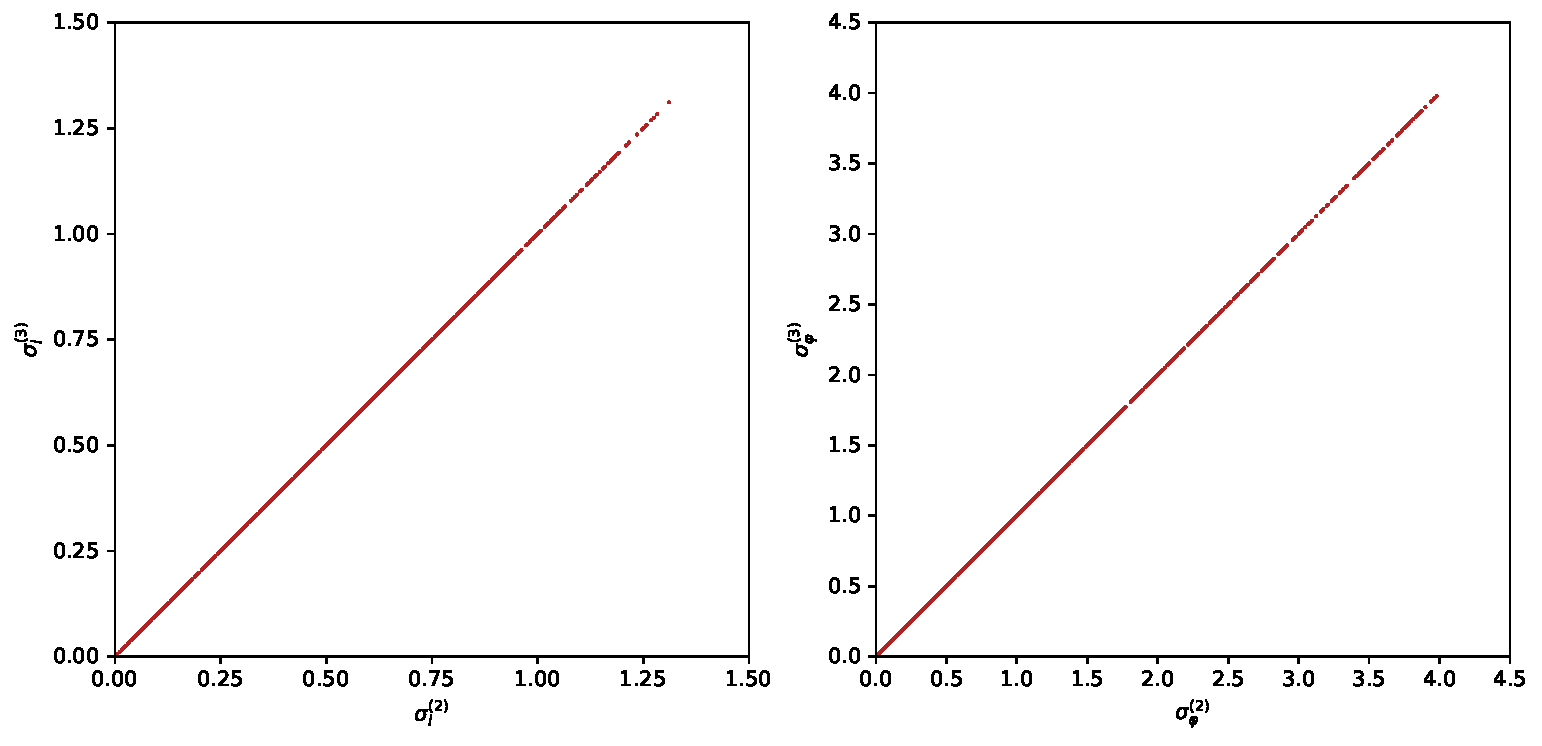
\includegraphics[width = 129.5mm]{figures/sv-sv.pdf}
    \caption[Ovisnosti druge i treće singularne vrijednosti duljina stranica odnosno vanjskih kutova na trokutima dijametra \ensuremath{\numprint{1}}]{Ovisnosti druge i treće singularne vrijednosti duljina stranica odnosno vanjskih kutova na trokutima dijametra \ensuremath{\numprint{1}}. Vektor \ensuremath{\sigma_{l} = \left( \sigma_{l}^{\left( \numprint{1} \right)} , \sigma_{l}^{\left( \numprint{2} \right)} , \sigma_{l}^{\left( \numprint{3} \right)} \right) \in \intervalco{\numprint{0}}{{+ \infty}}^{\numprint{3}}} vektor je singularnih vrijednosti duljina stranica, a vektor \ensuremath{\sigma_{\varphi} = \left( \sigma_{\varphi}^{\left( \numprint{1} \right)} , \sigma_{\varphi}^{\left( \numprint{2} \right)} , \sigma_{\varphi}^{\left( \numprint{3} \right)} \right) \in \intervalco{\numprint{0}}{{+ \infty}}^{\numprint{3}}} vektor je singularnih vrijednosti vanjskih kutova (uređeni su silazno tako da se svaka singularna vrijednost pojavljuje onoliko puta kolika joj je kratnost).}
    \label{fig:2_3_singular_value}
\end{figure}

\par

Osim spomenutih korelacija, proučavane su i \emph{složenije} korelacije tako da se od dvije značajke izračuna nova, treća značajka i onda proučava njezina korelacija s najmanjom svojstvenom vrijednosti. Od takvih proučavanih korelacija najbolje rezultate imale su značajke definirane s
\begin{align*}
    f_{\numprint{1}} \left( a , b \right) & \coloneqq \sqrt{\left( \frac{a}{A} \right)^{\numprint{2}} + \left( \frac{b}{B} \right)^{\numprint{2}}} \text{,} \\
    f_{\numprint{2}} \left( a , b \right) & \coloneqq \sqrt{\left( \frac{a}{A} \right)^{\numprint{2}} + \left( \frac{B - b}{B} \right)^{\numprint{2}}} \text{,} \\
    f_{\numprint{3}} \left( a , b \right) & \coloneqq \sqrt{\left( \frac{A - a}{A} \right)^{\numprint{2}} + \left( \frac{b}{B} \right)^{\numprint{2}}} \text{,} \\
    f_{\numprint{4}} \left( a , b \right) & \coloneqq \sqrt{\left( \frac{A - a}{A} \right)^{\numprint{2}} + \left( \frac{B - b}{B} \right)^{\numprint{2}}} \text{,}
\end{align*}
gdje su $ a , b $ vrijednosti nekih originalnih značajki (na primjer, drugi najveći vanjski kut ili najveća singularna vrijednost duljina stranica), a $ A , B $ najveće opažene vrijednosti tih značajki u skupu podataka za treniranje (mogu biti teorijski izračunate vrijednosti ako je poznat maksimum ili supremum promatrane značajke, kao, na primjer, $ \pi $ za najveći vanjski kut). Definirane značajke možemo shvatiti kao euklidske norme točaka u ravnini čije su koordinate dane izrazima $ \frac{a}{A} $ ili $ \frac{A - a}{A} $ i $ \frac{b}{B} $ ili $ \frac{B - b}{B} $. Značajke su u tim izrazima normirane zato što različite značajke imaju različite raspone vrijednosti pa kvadriranjem veća od tih značajki još jače dominira u izrazu $ a^{\numprint{2}} + b^{\numprint{2}} $. Ovisnosti najmanje svojstvene vrijednosti Laplaceovog operatora o dvama ovakvim značajkama dobivenim od druge najveće singularne vrijednosti duljina stranica i druge najveće singularne vrijednosti vanjskih kutova prikazane su na slici~\ref{fig:norm_singular_value_singular_value_eigenvalue}.

\par

\begin{figure}[htb!]
    \centering
    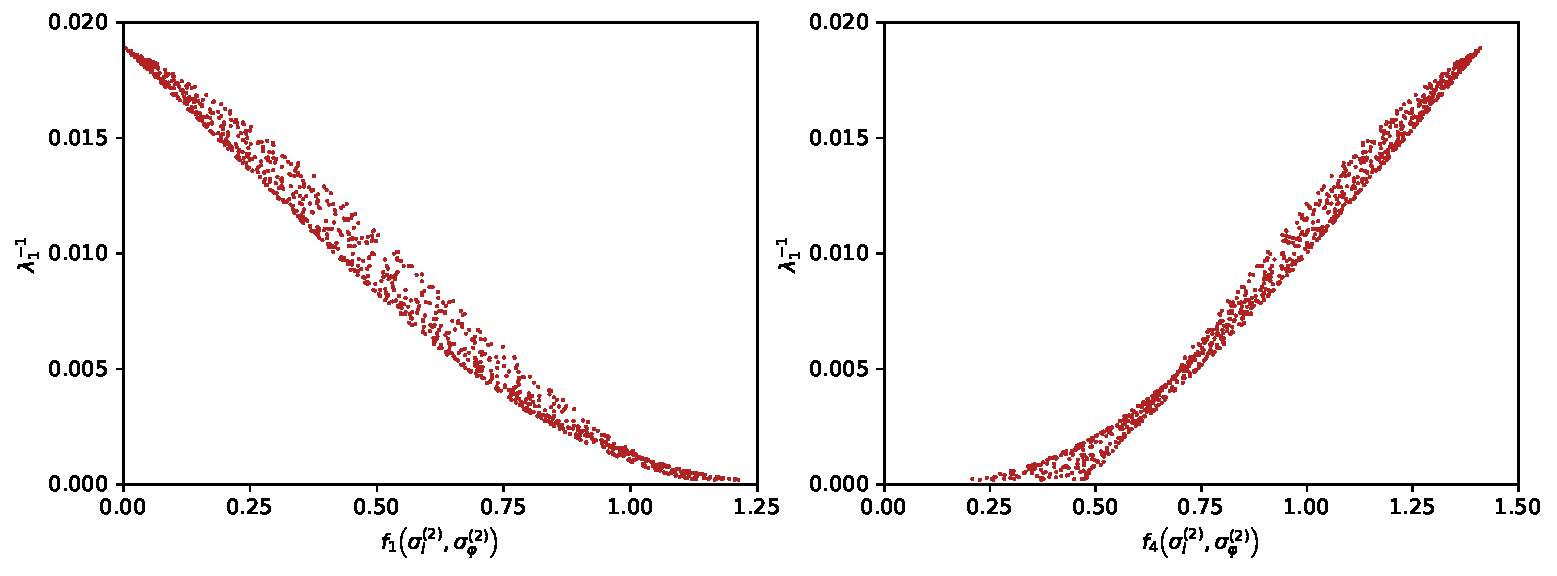
\includegraphics[width = 132mm]{figures/r(sv,sv)-lambda.pdf}
    \caption[Ovisnosti multiplikativnog inverza najmanje svojstvene vrijednosti Laplaceovog operatora na trokutima dijametra \ensuremath{\numprint{1}} u odnosu na dodatne složene značajke]{Ovisnosti multiplikativnog inverza najmanje svojstvene vrijednosti Laplaceovog operatora na trokutima dijametra \ensuremath{\numprint{1}} u odnosu na dodatne složene značajke \ensuremath{f_{\numprint{1}}} i \ensuremath{f_{\numprint{4}}} dobivene od druge najveće singularne vrijednosti duljina stranica i druge najveće singularne vrijednosti vanjskih kutova. Vektor \ensuremath{\sigma_{l} = \left( \sigma_{l}^{\left( \numprint{1} \right)} , \sigma_{l}^{\left( \numprint{2} \right)} , \sigma_{l}^{\left( \numprint{3} \right)} \right) \in \intervalco{\numprint{0}}{{+ \infty}}^{\numprint{3}}} vektor je singularnih vrijednosti duljina stranica, a vektor \ensuremath{\sigma_{\varphi} = \left( \sigma_{\varphi}^{\left( \numprint{1} \right)} , \sigma_{\varphi}^{\left( \numprint{2} \right)} , \sigma_{\varphi}^{\left( \numprint{3} \right)} \right) \in \intervalco{\numprint{0}}{{+ \infty}}^{\numprint{3}}} vektor je singularnih vrijednosti vanjskih kutova (uređeni su silazno tako da se svaka singularna vrijednost pojavljuje onoliko puta kolika joj je kratnost).}
    \label{fig:norm_singular_value_singular_value_eigenvalue}
\end{figure}

\par

Od složenih značajki (ali proučavale su se samo one dobivene od duljina stranica, vanjskih kutova i singularnih vrijednosti, a bez koordinata točke u skupu $ D_{{\bigtriangleup}} $) čak $ \numprint{55} $ ih je imalo Pearsonov koeficijent korelacije s najmanjom svojstvenom vrijednosti Laplaceovog operatora po apsolutnoj vrijednosti veći od $ \unit[\numprint{90}]{\%} $, ali među njima su uglavnom dominirale iste originalne značajke koje i samostalno imaju apsolutno visoke koeficijente korelacije. Apsolutno veći od $ \unit[\numprint{95}]{\%} $ koeficijent korelacije imale su $ \numprint{34} $ značajke, apsolutno veći od $ \unit[\numprint{99}]{\%} $ njih $ \numprint{6} $, a najveći (po apsolutnoj vrijednosti) je koeficijent korelacije značajke $ f_{\numprint{3}} $ od najvećeg vanjskog kuta i najveće singularne vrijednosti duljina stranica, koji iznosi $ \unit[\numprint{99.4679}]{\%} $.

\par

Međutim, takve i složenije značajke u konačnom su se rješenju izbjegavale zato da dobiveni modeli budu što interpretativniji, generalizabilniji i neartificijelniji. Za rješavanje drugačijeg problema, ali također diferencijalne jednadžbe, Mills i dr.\ u~\cite{bib:Mills17} uopće nisu koristili vlastite izabrane numeričke značajke, nego su konstruirali uspješni model koji sam pronalazi značajke iz vizualnog prikaza dvodimenzionalnih elektrostatskih potencijala.

\par
